\section{Operations of a heap}
\label{sec:operations_of_a_heap}

\begin{frame}
	\frametitle{Bubbles!}
	\begin{center}
		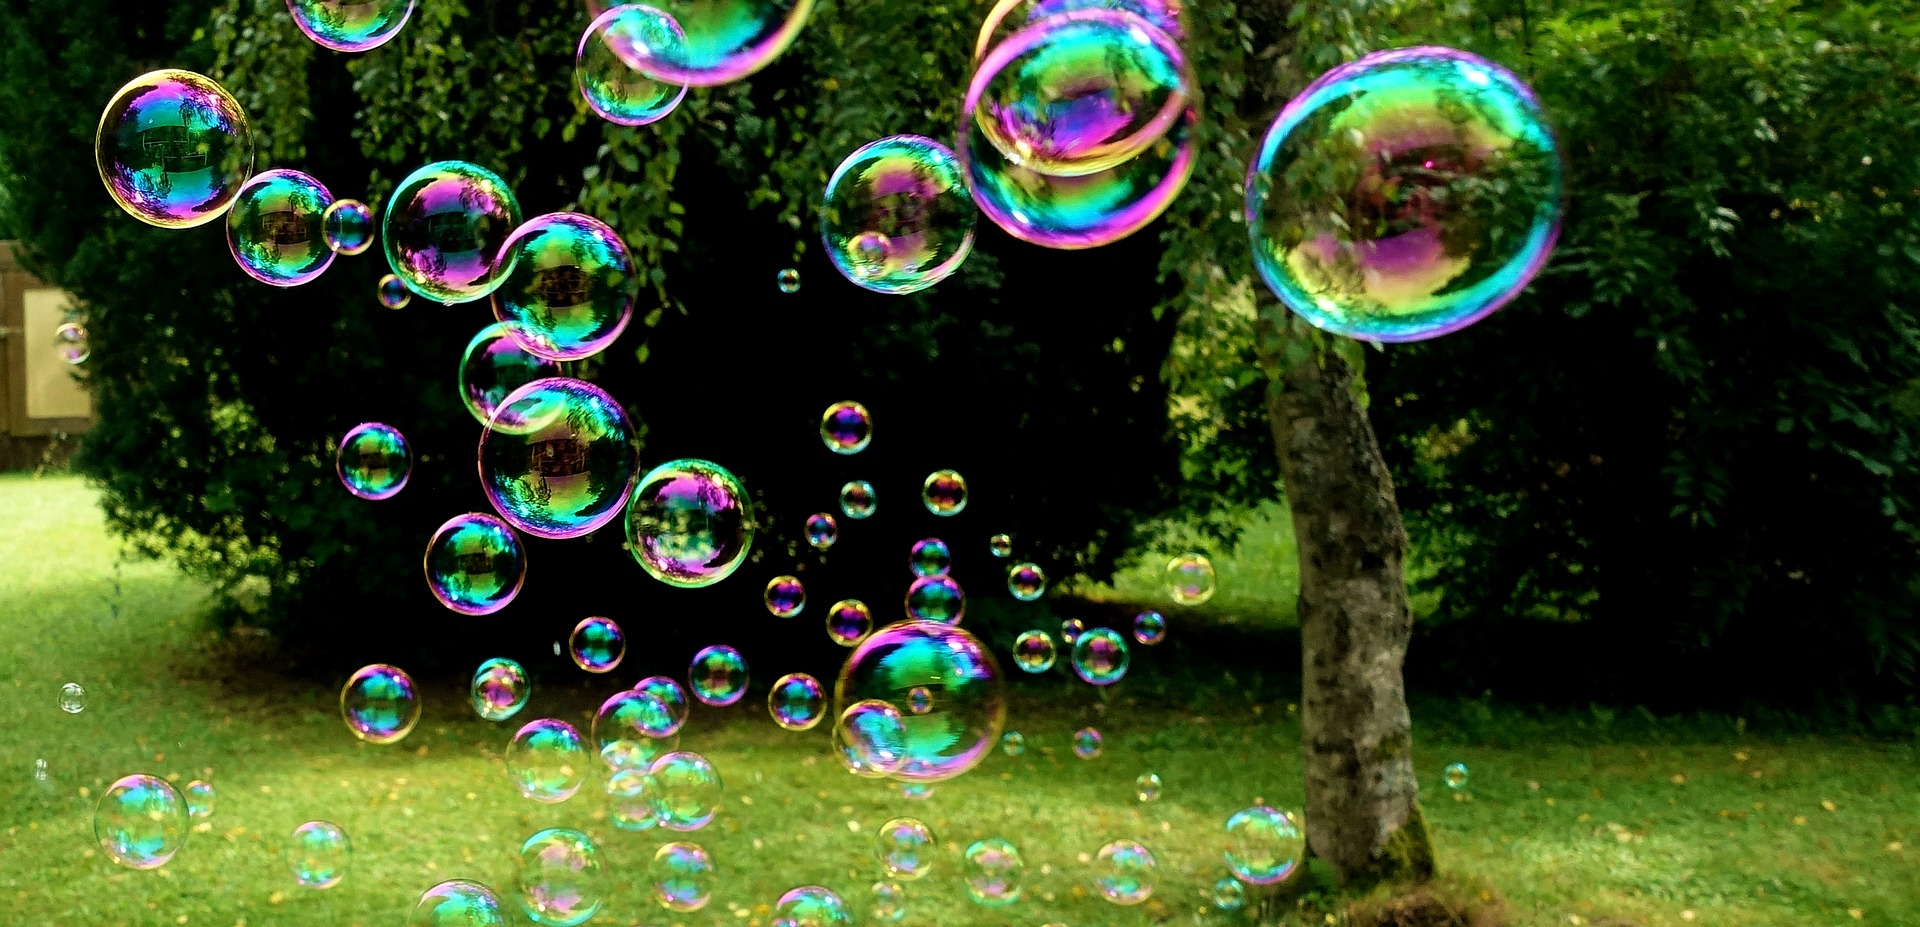
\includegraphics[width=0.8\textwidth]{figures/bubble.jpg}\\
		\hspace*{15pt}\hbox{\scriptsize Image By:\thinspace{\itshape Alexas Fotos}}
		% https://pixabay.com/photos/soap-bubbles-colorful-flying-3517247/
	\end{center}
\end{frame}

\begin{frame}
	\frametitle{\alt<2->{A PriorityQueue ADT}{A Heap ADT}}
		\begin{block}{Heap, Heap, Array}
			There is no heap ADT per sé, it's just a special type of tree.
		\end{block}	
		\pause
		\begin{block}{PriorityQueue}
			But there is one for a PriorityQueue (which we could implement using a heap):
			\begin{itemize}
				\item \texttt{size()} (or \texttt{len} in Python) to get the number of elements.
					\pause
				\item \texttt{add(item)} to insert an item into the queue.
					\pause
				\item \texttt{remove\_min()} to remove the smallest element from the queue.
					\pause
				\item \texttt{min()} to get the smallest element from the queue.
			\end{itemize}
		\end{block}	
\end{frame}

\begin{frame}
	\frametitle{An array-based Priority Queue}

	\vspace{-20pt}
	\begin{columns}[t]
		\column{0.455\textwidth}
		\lstinputlisting{code/pq_array.py}
		\column{0.455\textwidth}
		\pause
		\begin{exampleblock}{Array-based PQ}
			We can easily create a PQ based on an array (or list).
		\end{exampleblock}	
		\pause
			\begin{alertblock}{No, bad line graph!}
				But this makes \texttt{min} and \texttt{remove\_min} linear time operations!
			\end{alertblock}	
			\pause
			\begin{questionblock}{Can we do better?}
				Can we do better by using a sorted array?
			\end{questionblock}
	\end{columns}
\end{frame}

\begin{frame}
	\frametitle{An sorted array-based Priority Queue}

	\vspace{-20pt}
	\begin{columns}[t]
		\column{0.455\textwidth}
		\lstinputlisting{code/pq_sortedarray.py}
		\column{0.455\textwidth}
		\pause
		\begin{exampleblock}{Array-based PQ}
			We can easily create a PQ based on a sorted array (or list).
		\end{exampleblock}	
		\pause
			\begin{alertblock}{No, bad line graph!}
				But this makes \texttt{remove\_min} and \texttt{add} linear time operations!
			\end{alertblock}	
			\pause
			\begin{questionblock}{Can we do better?}
				Can we do better by using a heap?
			\end{questionblock}
	\end{columns}
\end{frame}

\begin{frame}
	\frametitle{Min in a heap}
	\begin{questionblock}{Consider a heap}
		How do I implement \texttt{min} for my heap-based PQ?
		\begin{enumerate}[A.]
			\item Return the value in the root.
			\item Return the value of the left-most descendant.
			\item Return the value of the right-most descendant.
			\item Go over all elements and return the minimum.
		\end{enumerate}
	\end{questionblock}
	
	
\end{frame}

\begin{frame}
	\frametitle{Adding in a heap}
	\begin{questionblock}{Consider a heap}
		Consider the following heap:\\
		\begin{columns}
			\column{0.455\textwidth}
			\begin{tikzpicture}[
				level distance = 2.5em,
				level 1/.style={sibling distance=9em},
				level 2/.style={sibling distance=4.5em},
				level 3/.style={sibling distance=2.25em},
				]
				\node[ellipse] (t1) {1}
				child { node[ellipse]   {12}
					child { node[ellipse] {14}}
					child { node[ellipse] {17}}
				}
				child { node[ellipse]   {4}
					child { node[ellipse] {5}}
				};
			\end{tikzpicture}
			\column{0.455\textwidth}
			\pause
			If I insert the element $7$ here, what should I do?
		\end{columns}
	\end{questionblock}
	\begin{answerblock}{Just add it at the bottom-right!}
			\begin{tikzpicture}[
				level distance = 2.5em,
				level 1/.style={sibling distance=9em},
				level 2/.style={sibling distance=4.5em},
				level 3/.style={sibling distance=2.25em},
				scale=0.8, transform shape
				]
				\node[ellipse] (t1) {1}
				child { node[ellipse]   {12}
					child { node[ellipse] {14}}
					child { node[ellipse] {17}}
				}
				child { node[ellipse]   {4}
					child { node[ellipse] {5}}
					child { node[ellipse] {7}}
				};
			\end{tikzpicture}
	\end{answerblock}
\end{frame}

\begin{frame}
	\frametitle{Adding in a heap}
	\begin{questionblock}{Consider a heap}
		Consider the following heap:\\
		\begin{columns}
			\column{0.455\textwidth}
			\begin{tikzpicture}[
				level distance = 2.5em,
				level 1/.style={sibling distance=9em},
				level 2/.style={sibling distance=4.5em},
				level 3/.style={sibling distance=2.25em},
				]
				\node[ellipse] (t1) {1}
				child { node[ellipse]   {12}
					child { node[ellipse] {14}}
					child { node[ellipse] {17}}
				}
				child { node[ellipse]   {4}
					child { node[ellipse] {5}}
				};
			\end{tikzpicture}
			\column{0.455\textwidth}
			\pause
			If I insert the element $0$ here, what should I do?
		\end{columns}
	\end{questionblock}
	\begin{alertblock}{Just add it at the bottom-right!}
		\begin{columns}
			\column{0.455\textwidth}
			\begin{tikzpicture}[
				level distance = 2.5em,
				level 1/.style={sibling distance=9em},
				level 2/.style={sibling distance=4.5em},
				level 3/.style={sibling distance=2.25em},
				scale=0.8, transform shape
				]
				\node[ellipse] (t1) {1}
				child { node[ellipse]   {12}
					child { node[ellipse] {14}}
					child { node[ellipse] {17}}
				}
				child { node[ellipse]   {4}
					child { node[ellipse] {5}}
					child { node[ellipse] {0}}
				};
			\end{tikzpicture}
			\column{0.455\textwidth}
			\pause
			And now fix the damage we have caused :)
		\end{columns}
	\end{alertblock}
\end{frame}

\begin{frame}
	\frametitle{Up-bubbling}

	\begin{problemblock}{Fixing the damage}
		How can we fix the damage caused to the heap \textit{efficiently}?
		\begin{columns}
			\column{0.455\textwidth}
			\begin{tikzpicture}[
				level distance = 2.5em,
				level 1/.style={sibling distance=9em},
				level 2/.style={sibling distance=4.5em},
				level 3/.style={sibling distance=2.25em},
				scale=0.8, transform shape
				]
				\node[ellipse] (t1) {1}
				child { node[ellipse]   {12}
					child { node[ellipse] {14}}
					child { node[ellipse] {17}}
				}
				child { node[ellipse]   {4}
					child { node[ellipse] {5}}
					child { node[ellipse] {0}}
				};
			\end{tikzpicture}
			\column{0.455\textwidth}
			\pause
			\begin{enumerate}[A.]
				\item Swap it with the root element and then swap it down as needed.
				\item Repeatedly compare the new node with the siblings and swap if needed.
				\item Repeatedly compare the new node with the parent and swap if needed.
				\item We cannot, we have to rebuild the entire heap.
			\end{enumerate}
		\end{columns}
	\end{problemblock}
\end{frame}

\begin{frame}
	\frametitle{Up-bubbling}

	\begin{answerblock}{Fixing the damage}
		Repeatedly switch with the parent if needed.\\
		\begin{columns}
			\column{0.455\textwidth}
				
			\begin{tikzpicture}[
				level distance = 2.5em,
				level 1/.style={sibling distance=9em},
				level 2/.style={sibling distance=4.5em},
				level 3/.style={sibling distance=2.25em},
				scale=0.8, transform shape
				]
				\node[ellipse,onslide=<4-5>{draw=red}] (t1) {\alt<5->{\alert<5>{0}}{1}}
				child { node[ellipse]   {12}
					child { node[ellipse] {14}}
					child { node[ellipse] {17}}
				}
				child { node[ellipse,onslide=<2-5>{draw=red}] {\alt<5->{\alert<5>{1}}{\alt<3->{\alert<3>{0}}{4}}}
					child { node[ellipse] {5}}
					child { node[ellipse,onslide=<2-3>{draw=red}] {\alt<3->{\alert<3>{4}}{0}}}
				};
			\end{tikzpicture}
			\column{0.455\textwidth}
			\only<6->{
			\begin{itemize}
				\item Notice how the left half of the tree has not been touched at all!
				\item Only one path changes!
			\end{itemize}	
	}
		\end{columns}
	\end{answerblock}
\end{frame}

\begin{frame}
	\frametitle{Up-bubbling pt2}
			\begin{tikzpicture}[
				level distance = 2.5em,
				level 1/.style={sibling distance=9em},
				level 2/.style={sibling distance=4.5em},
				level 3/.style={sibling distance=2.25em},
				scale=0.8, transform shape
				]
				\node[ellipse] (t1) {6}
				child { node[ellipse]   {14}
					child { node[ellipse] {17}}
					child { node[ellipse] {21}}
				}
				child { node[ellipse]   {8}
					child { node[ellipse] {18}}
					child { node[ellipse] {9}}
				};
			\end{tikzpicture}
			\begin{questionblock}{Where does it go?}
				Try to insert the element $10$ in this heap. Where does it end up?
				\begin{enumerate}[A.]
					\item As the root
					\item At depth 1
					\item At depth 2
					\item At depth 3
				\end{enumerate}
			\end{questionblock}
\end{frame}

\begin{frame}
	\frametitle{Removing from a heap}
	\begin{questionblock}{Consider a heap}
		Consider the following heap:\\
		\begin{columns}
			\column{0.455\textwidth}
			\begin{tikzpicture}[
				level distance = 2.5em,
				level 1/.style={sibling distance=9em},
				level 2/.style={sibling distance=4.5em},
				level 3/.style={sibling distance=2.25em},
				]
				\node[ellipse] (t1) {1}
				child { node[ellipse]   {12}
					child { node[ellipse] {14}}
					child { node[ellipse] {17}}
				}
				child { node[ellipse]   {4}
					child { node[ellipse] {5}}
					child { node[ellipse] {7}}
				};
			\end{tikzpicture}
			\column{0.455\textwidth}
			\pause
			If I want to remove the minimum, what should I do?
		\end{columns}
	\end{questionblock}
	\begin{alertblock}{Just remove it at the top!}
		\begin{columns}
			\column{0.455\textwidth}
			\begin{tikzpicture}[
				level distance = 2.5em,
				level 1/.style={sibling distance=9em},
				level 2/.style={sibling distance=4.5em},
				level 3/.style={sibling distance=2.25em},
				scale=0.8, transform shape
				]
				\node[ellipse] (t1) {$\square$}
				child { node[ellipse]   {12}
					child { node[ellipse] {14}}
					child { node[ellipse] {17}}
				}
				child { node[ellipse]   {4}
					child { node[ellipse] {5}}
					child { node[ellipse] {7}}
				};
			\end{tikzpicture}
			\column{0.455\textwidth}
			\pause
			And now fix the damage we have caused :)
		\end{columns}
	\end{alertblock}
\end{frame}

\begin{frame}
	\frametitle{Fixing the damage}
	\begin{questionblock}{Just remove it at the top!}
		\begin{columns}
			\column{0.455\textwidth}
			\begin{tikzpicture}[
				level distance = 2.5em,
				level 1/.style={sibling distance=9em},
				level 2/.style={sibling distance=4.5em},
				level 3/.style={sibling distance=2.25em},
				scale=0.8, transform shape
				]
				\node[ellipse] (t1) {$\square$}
				child { node[ellipse]   {12}
					child { node[ellipse] {14}}
					child { node[ellipse] {17}}
				}
				child { node[ellipse]   {4}
					child { node[ellipse] {5}}
					child { node[ellipse] {7}}
				};
			\end{tikzpicture}
			\column{0.455\textwidth}
			\pause
			What should we do?
			\begin{enumerate}[A.]
				\item Repeatedly move the smallest child up.
				\item First move the bottom right to the root and then repeatedly swap down with the smallest child.
				\item Always get the smallest element from the next layer and move it up (so not restricted to your children).
				\item Nothing, we should just rebuild the heap from scratch.
			\end{enumerate}
		\end{columns}
	\end{questionblock}
	
\end{frame}

\begin{frame}
	\frametitle{Down-bubbling}

	\begin{answerblock}{Fixing the damage}
		First move the bottom-right element to the top, then repeatedly bubble down.
		\begin{columns}
			\column{0.455\textwidth}
				
			\begin{tikzpicture}[
				level distance = 2.5em,
				level 1/.style={sibling distance=9em},
				level 2/.style={sibling distance=4.5em},
				level 3/.style={sibling distance=2.25em},
				scale=0.8, transform shape
				]
				\node[ellipse,onslide=<2-5>{draw=red}] (t1) {\alt<5->{\alert<5>{4}}{{\alt<3->{\alert<3>{7}}{$\square$}}}}
				child { node[ellipse]   {12}
					child { node[ellipse] {14}}
					child { node[ellipse] {17}}
				}
				child { node[ellipse,onslide=<4-7>{draw=red}] {\alt<7->{\alert<7>{5}}{\alt<5->{\alert<5>{7}}{4}}}
					child { node[ellipse,onslide=<6-7>{draw=red}] {\alt<7->{\alert<7>{7}}{5}}}
					child { node[ellipse,onslide=<2-3>{draw=red}] {\alt<3->{\alert<3>{$\square$}}{7}}}
				};
			\end{tikzpicture}
			\column{0.455\textwidth}
			\only<8->{
			\begin{itemize}
				\item Notice how the left half of the tree has not been touched at all!
				\item Only one path changes, after the initial switch!
			\end{itemize}	
	}
		\end{columns}
	\end{answerblock}
\end{frame}

\begin{frame}
	\frametitle{Down-bubbling pt2}
			\begin{tikzpicture}[
				level distance = 2.5em,
				level 1/.style={sibling distance=9em},
				level 2/.style={sibling distance=4.5em},
				level 3/.style={sibling distance=2.25em},
				scale=0.8, transform shape
				]
				\node[ellipse] (t1) {6}
				child { node[ellipse]   {14}
					child { node[ellipse] {17}
						child { node[ellipse] {19}}
					}
					child { node[ellipse] {21}
					}
				}
				child { node[ellipse]   {8}
					child { node[ellipse] {18}}
					child { node[ellipse] {12}
					}
				};
			\end{tikzpicture}
			\begin{questionblock}{Where does it go?}
				Remove the minimum from the heap, where does $18$ end up?
				\begin{enumerate}[A.]
					\item As the root
					\item At depth 1
					\item At depth 2
					\item At depth 3
				\end{enumerate}
			\end{questionblock}
\end{frame}
